% Tento soubor nahraďte vlastním souborem s obsahem práce.
%=========================================================================
% Autoři: Michal Bidlo, Bohuslav Křena, Jaroslav Dytrych, Petr Veigend a Adam Herout 2019

% Pro kompilaci po částech (viz projekt.tex), nutno odkomentovat a upravit
%\documentclass[../projekt.tex]{subfiles}
%\begin{document}

\chapter{Úvod}
%cca strana

\chapter{Teoretická část} %přejmenovat

\section{Hardware Adeept AWR 4WD a Raspberry Pi}
Celá práce je implementována nad existujícím hardwarem. Konkrétně se jedná o "stavebnici" Adeept AWR 4WD z níž pochází všechny periferie, jako motory, serva a čidla. Tyto periferie jsou pak ovládány mikropočítačem Raspberry Pi4. V porovnání s běžně používanými mikrokontrolery se jedná o výkonější hardware.

\subsection*{Adeept AWR 4WD}

\subsubsection*{Robot HAT}
Adeept Robot HAT je hardwarová deska, která slouží k rozšíření Rapsberry Pi o další funkcionalitu. K rpi se připojuje pomocí GPIO(General purpuse input outpu) pinů. Deska jako taková obsahuje rozšiřující čipy a rozhraní sloužící k ovládání připojených periferií.

\begin{itemize}
	\item{PCA9685 \cite{pca9685}}
	\begin{itemize}
		\item{generátor PWM signálu}
		\item{16 kanálů}
		\item{12 bitů rozlišení střídy (4096 možných hodnot)}
		\item{je ovládaný přes I2C sběrnici}
	\end{itemize}
	\item{L298P}
	\begin{itemize}
		\item{ovladač pro řízení dc motoru}
		\item{obsahuje full bridge obvod (viz následující obrázek)}
		\item{umožňuje roztočit motor oběma směry}
		\item{pomocí PWM lze ovládat rychlost motorů}
	\end{itemize}
	\item{další rozhraní pro připojení periferií (ultrasonic sensor, line tracking)}
\end{itemize}

\begin{figure}[h!]
	\centering
	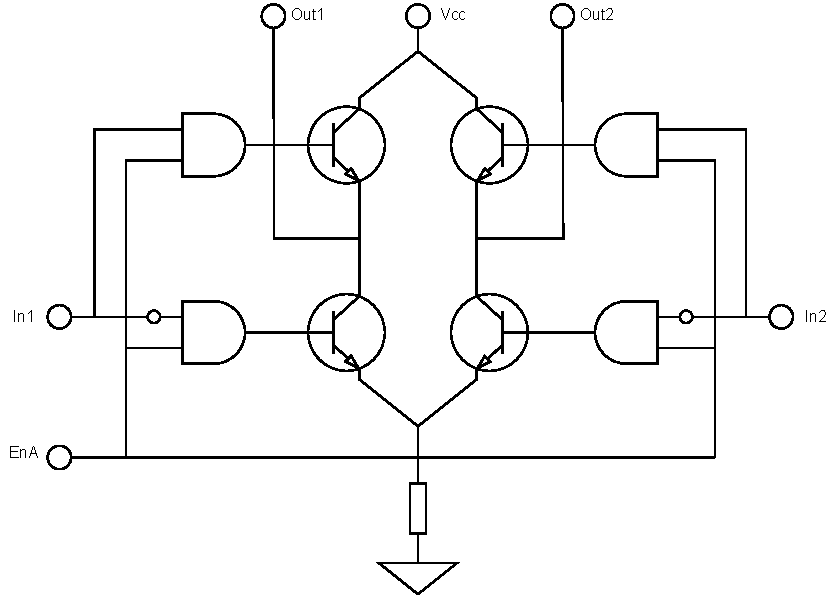
\includegraphics[scale=0.75]{obrazky-figures/motor_full_bridge.pdf}
	\caption{Full bridge konfigurace pro ovládání motoru. In1 a In2 určují směr otáčení. EnA je PWM signál určující rychlost otáčení. \cite{l298}}
	\label{}
\end{figure}

%batery - napájení

\subsubsection{I2C}
Je synchronní sběrnice, která se vyznačuje svou jednoduchostí a nízkou cenou. Využívá dva vodiče SDA (serial data) a SCL (serial clock). Oba vodiče jsou připojeny k napájecímu napětí pomocí pull-up rezistoru a bez vlivu jiného hardwaru zůstávají v logické jedničce. Zařízení která jsou na tuto sběrnici připojeny využívají open drain k úpravě aktuální napěťové úrovně na sběrnici. I2C pak pracuje s dvěma druhy zařízení, master a slave. Master zahajuje a ukončuje komunikaci, typicky se jedná o mikrokontroler. Slave jsou pak ostatní zařízení s nimiž může master komunikovat, typicky různé periferie. \cite{um10204}

\begin{figure}[h!]
	\centering
	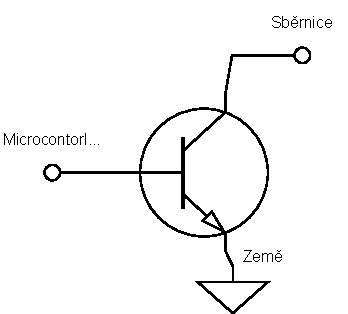
\includegraphics[scale=0.75]{obrazky-figures/open_drain.pdf}
	\caption{Open drain}
	\label{}
\end{figure}

Přenos jednoho datového rámce zahájí master zařízení přivedením datové sběrnice do nuly. Následující komunikace se skládá z odeslání rámce o délce osmi bitů a potvrzení o úspěšném přenosu dat od přijímajícího zařízení. Toto potvrzení se nazývá ACK a je provedeno podržením datové sběrnice v hodnotě nula po dobu jednoho taktu. Opačný stav se nazývá NACK a indikuje že došlo k chybě. Ukončení přenosu je provedeno navrácením datové sběrnice na hodnotu jedna.

\begin{figure}[h!]
	\centering
	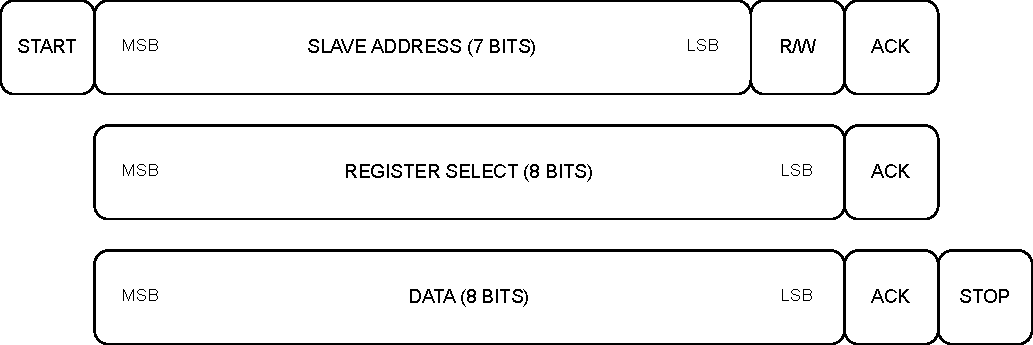
\includegraphics[scale=0.75]{obrazky-figures/i2c_data_word.pdf}
	\caption{Na obrázku lze vidět, jak může vypadat přenos jednoho datového slova. V prvním rámci je přenesena sedmi bitová adresa sloužící k výběru slave zařízení se kterým chce máster navázat komunikaci. Doplněná o jeden bit indikující směr, kterým potečou data. V druhém rámci dojde k adresaci konkrétního registru a ve třetím se pošlou samotná data. \cite{an4481}}
	\label{}
\end{figure}

\subsubsection*{Pulzně šířková modulace}
Jedná se o techniku která umožňuje vytvořit pseudo-analogový výstup s použitím digitálních pinů. Mikrokontrolery jsou digitální zařízení a chtěly by tedy s okolním světem komunikovat pomocí digitálních pinů. Reálný svět však nefunguje pouze na úrovni jedniček a nul a je poroto potřeba převádět výstup z mikrokontroleru na analogový signlál. Problém je v tom, že převod digitálního signálu na analogový je relativně dlouhá a neefektivní operace. Proto vznikla pulzně šířková modulace, která umožňuje relativně jednoduše simulovat analogový výstup.

Při pohledu na klasický digitální signál který rovnoměrně střídá vysokou a nízkou úroveň by šlo říci, že se jedná o PWM signál se střídou 50\%. Střída udává poměr času kdy je signál v logické jedničce ku času kdy je v nule. Součet těchto hodnot se musí rovnat délce jedné periody. Úpravou tohoto poměru lze simulovat analogový signál.

\begin{figure}[h!]
	\centering
	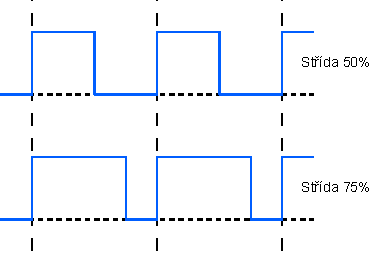
\includegraphics[scale=1]{obrazky-figures/pwm_duty_cycle.pdf}
	\caption{Signál pro různé hodnoty střídy}
	\label{}
\end{figure}

\subsubsection*{DC Motor}
Pohyb celého autíčka zajišťují čtyři motory. Jsou napájeny pomocí stejnosměrného proudu(dc - direct current). K jejich ovládání a dodání většího proudu než je schopno poskytnout raspberry pi slouží obvod L298P který je součástí Robot HAT.
Elektrický DC motor se skládá ze dvou hlavních částí, stator a rotor. Stator je statická, vnější část, a typicky se jedná o permanentní magnet. Uvnitř statoru se pak nachází rotor, ten se skládá z elektromagnetů, které při zapnutí reagují s statorem(póly se odpuzují a přitahují) a dojde tak k částečnému pootočení. Při správném spínání a vypínání těchto magnetů lze motor rozběhnout. To zajišťuje komutátor, jedná se o prstenec složený z několika navzájem odizolovaných částí, které jsou připojeny na vývody elektromagnetu. S povrchem prstence jsou pomocí pružin v kontaktu dva kartáče, které jsou připojeny na napájení a zemi. Komutátor se otáčí společně s rotorem a při tomto pohybu se kartáče postupně dotýkají různých částí komutátoru a spínají tak jednotlivé elektromagnety, ty vedou k pootočení rotoru a sepnutí následujícího magnetu.

\begin{figure}[h!]
	\centering
	%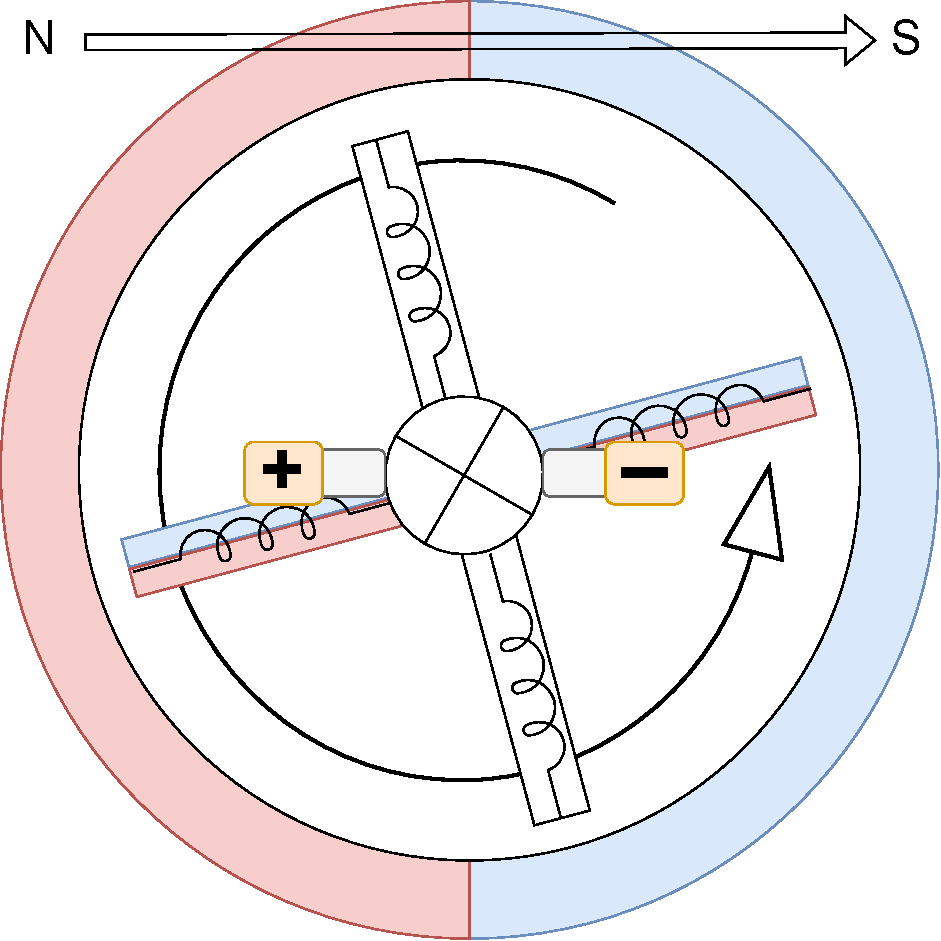
\includegraphics[scale=1]{obrazky-figures/dc_motor.pdf}
	\caption{Signál pro různé hodnoty střídy}
	\label{}
\end{figure}

Dc motor má stator, permanentní magnet. A rotor, cívky do kterých se pak posílá proud tak aby se od statoru odpuzovaly a roztáčí se tak rotor.

\subsubsection*{Led}

\subsubsection*{Servo}
Adeept AWD 4WD využívá pouze jedno servo, a to na ovládání úhlu kamery. Konkrétně se jedná o model Adeept AD002. Je ovládané pomocí PWM signálu. Generování tohoto signálu zajišťuje čip PCA9685 který je umístěný na Robot HAT.

\subsubsection*{Depth module}
%hc-sr04
Funguje na principu radaru. Vyšle zvukovou vlnu na frekvenci 40Khz %je v tutorialu adeept
 a uloží si časovou značku. Následně poslouchá než se mu vlna vrátí a tehdy uloží druhou značku. Kdyz pak ví jak rychle se šíří zvuk ve vzduchu dokáže vypočítat vzdálenost od překážky.

$$S = (T_2 - T_1) * V_S / 2$$
Kde $T_1$ je moment kdy byla vyslána vlna $T_2$ kdy byla vlna přijata a $V_S$ rychlost šíření zvuku ve vzduchu.

\subsubsection*{Line tracking}
Funguje podobne jako depth module. Vysílá ultračervené tentokrát světlo a sleduje jestli došlo k odrazu. Bílý papír většinu světla odrazí a senzor jej zachytí, naopak černá čára světlo pohltí a senzor tak pozná že našel čáru.

\subsection*{Raspberry Pi 4b}
Jako mozek celého systému je použit mikropočítač Raspberry Pi. Konkrétně se jedná o verzi 4 model B s operační pamětí o velikostí čtyř gigabajtů. Tato verze obsahuje 64bitový procesor, který je potřeba pro spuštění 64 bitového Ubuntu serveru, který je doporučeným operačním systémem pro požití ROS2 na raspberry pi.
Komunikace s většinou použitých periferií je uskutečněna pomocí General Purpuse Input Output(GPIO) pinů. Jedná se o digitální vývody, které podle potřeby můžou fungovat jako vstup i výstup ze zařízení. Některé z nich pak mají ještě speciální funkce, například GPIO 2 a 3 můžou pracovat jako SDA a SCL připojení pro I2C komunikaci.

\begin{figure}[h!]
	\centering
	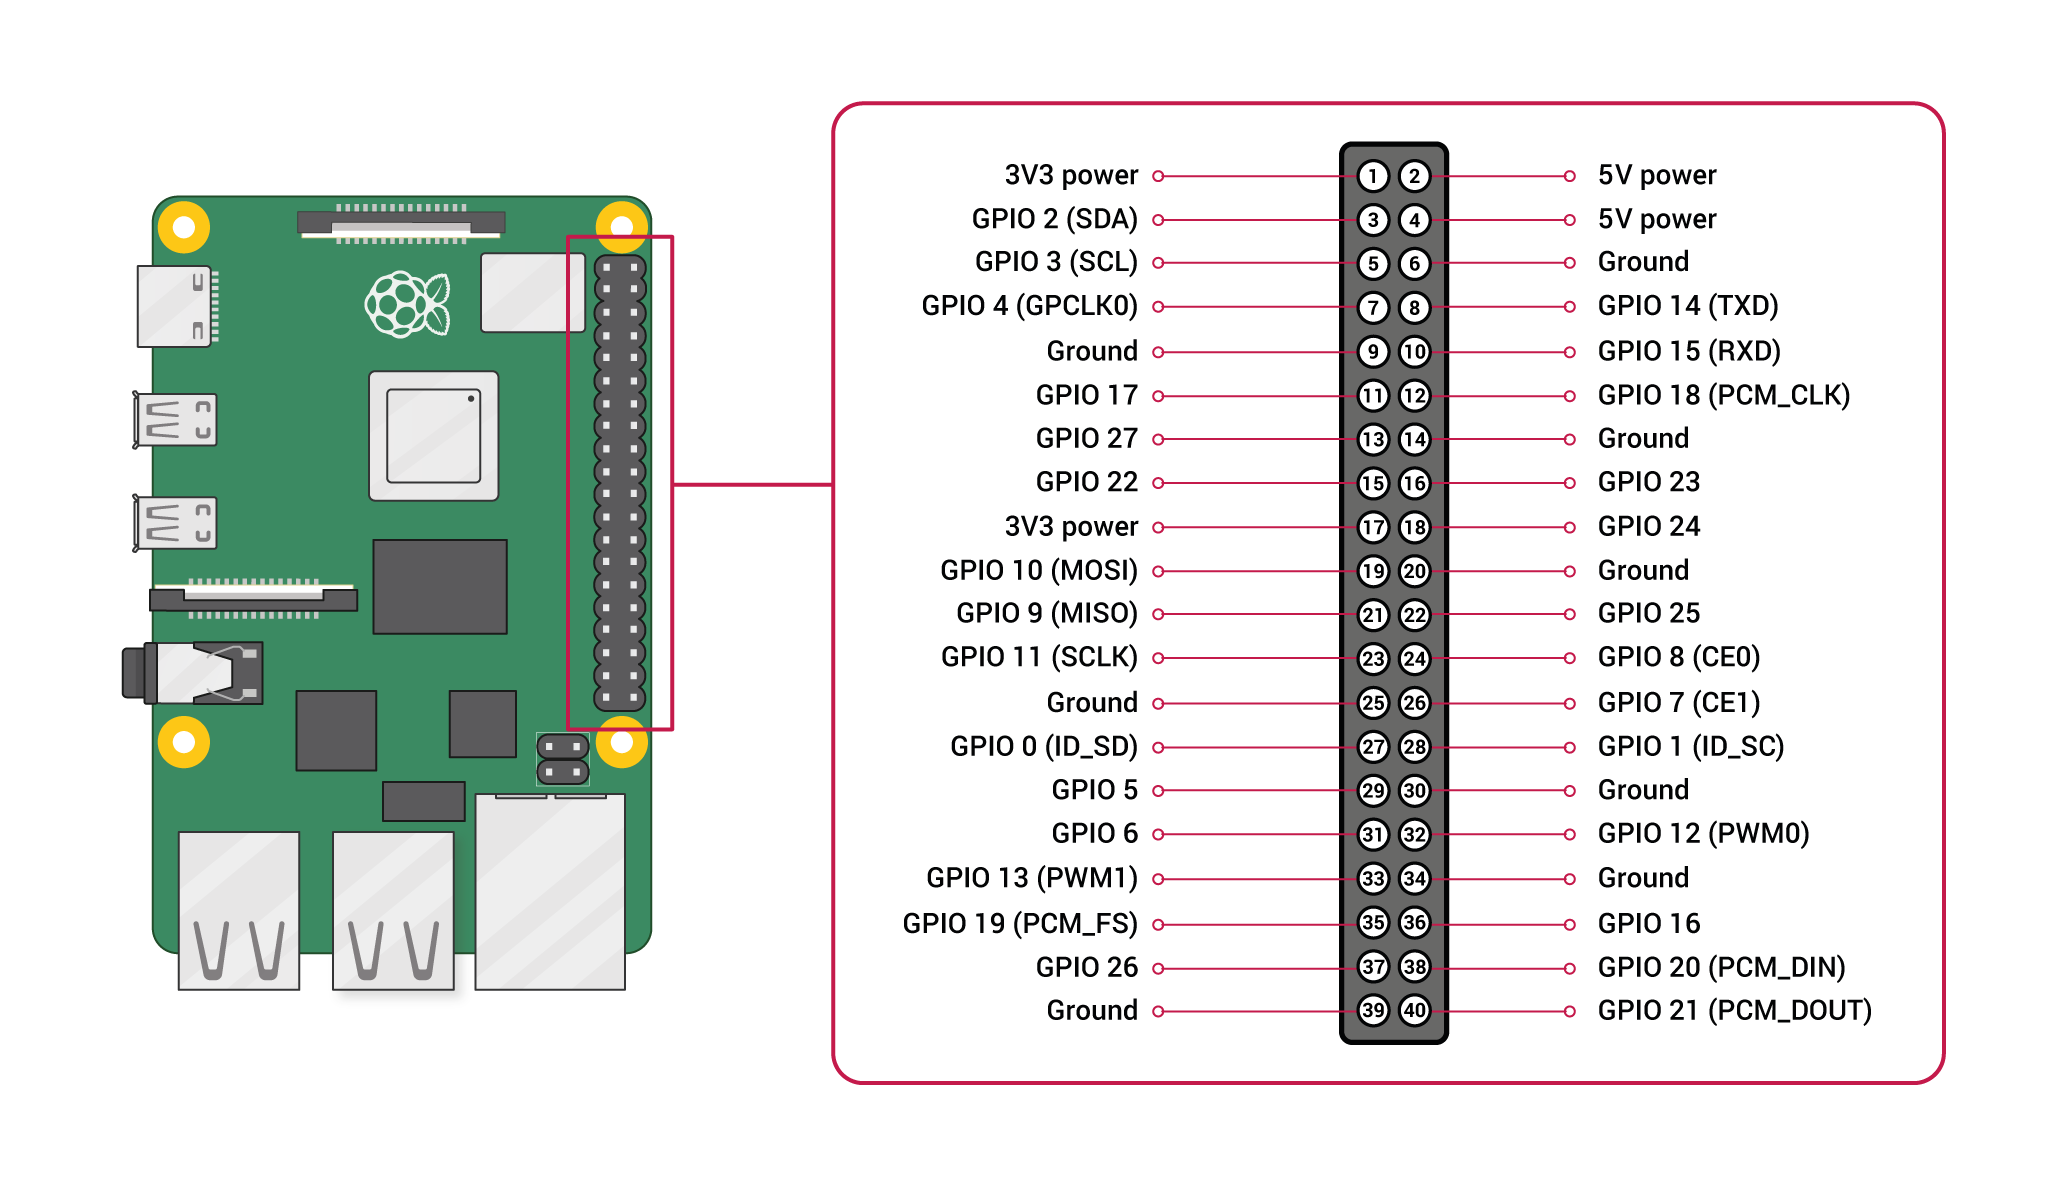
\includegraphics[scale=0.15]{obrazky-figures/gpio_pinout.png}
	\caption{GPIO pinout}
	\label{}
\end{figure}

\subsubsection*{Camera}

\section{Aktuální software}
Tento robot je dodáván s ukázkovým softwarem. Ten je implementován v jazyku python a využívá knihovny třetích stran sloužící k nízkoúrovňovému ovládání hardware komponent. Aby byl robot responzivní je celá implementace řešena s použitím python modulů sloužících k realizaci multithreadingu. Tento přístup bezpochyby funguje, avšak i u tohoto relativně malého projektu se takový kód stává poměrně složitým na porozumění.

%koncepce (multithreading, knihovny)

\


%zhodnocení (plánované změny a naopak ponechané části)

\section{Seznámení s ROS2} %cite knizku
ROS2 je middleware sloužící k vývoji a řízení robotů. Middleware je softwarová vrstva běžící nad operačním systémem sloužící k rozšíření jeho funkcionality. Typicky middleware obsahuje knihovny, ovladače, vývojové a monitorovací nástroje. Může také specifikovat doporučené metodologie pro vývoj. ROS2 je již druhá verze tohoto softwaru, která rozšiřuje a opravuje neduhy první verze. Původní ROS1 je považován za de-facto standart pro vývoj robotických aplikací.
Tato práce využívá ros2 distribuci jménem iron. Distribuce v ROS2 lze popsat jako set operačního systému, knihoven a dalších aplikací, které jsou otestovány a je zaručeno, že jsou navzájem kompatibilní. Velkou výhodou ROS je fakt, že se jedná o open source projekt. Díky tomu kolem něj vznikla velká komunita vývojářů, ale i firem a dalších institucí, které tvoří mnoho souvisejícího obsahu. Existuje tedy velké množství knihoven, dokumentací a návodů které usnadňují vývojářům práci.

\subsection*{Vrstvy ROS2}
Na nejvyšší úrovni, se nachází programátor který interaguje s klientskými knihovnami pro vývoj ROS2 aplikací. Tyto knihovny jsou oficiálně dvě a to rclpy pro python a rclcpp pro C++. Existují také implementace pro další programovací jazyky (rclc, java, C\#), ty jsou však udržovány komunitně. Všechny klientské knihovny pak využívají rcl. RCL je jádro celého ROS implementované v jazyce C. RCL implementuje hlavní ros2 funkcionalitu, kterou následně poskytuje pomocí rozhraní jednotlivým klientským knihovnám. Díky tomuto se funkcionalita implementovaná v pythonu bude chovat stejně jako ta implementovaná v c++. Taky pak kód implementovaný v c++ může komunikovat s tím v pythonu.
Poslední vrstvou je data distribution service. DDS je komunikační vrstva implementována na UDP protokolu sloužící k předávání informací mezi procesy. Má charakteristiky systémů reálného času, zajišťuje kvalitu a zabezpečení komunikace. Také umožňuje vyhledávání uzlů bez potřeby centralizovaného serveru (využívá k tomu multicast, komunikace mezi uzly je následně unicast).

\begin{figure}[h!]
	\centering
	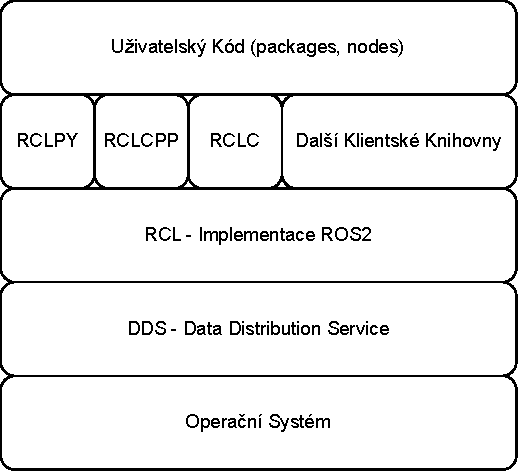
\includegraphics[scale=0.75]{obrazky-figures/ros_layers.pdf}
	\caption{Layers}
	\label{}
\end{figure}

\subsection{Vývoj v ROS2} %cite knizku
Nejvyšší organizační jednotkou v ROS2 je workspace. Jedná se o složku, která slouží k organizaci zdrojových souborů, jejich instalaci a následné spouštění. ROS2 instalace je také workspace a před použitím je potřeba ji nejprve aktivovat. K tomu v linuxu slouží příkaz \verb|source|. Aktivace workspace je akumulativní a v jeden moment tedy může být aktivních několik workspace. Typicky se první aktivuje základní ros2 instalace, která tvoří takzvanou underlay vrstvu. Vývojový workspace aktivovaný jako druhý se pak nazývá overlay. Pokud má overlay nějaké závislosti, měly by být uspokojeny v underlay.
Zdrojové soubory v rámci workspace jsou pak organizovány do packages. Package může obsahovat zdrojové soubory, knihovny a definice zpráv. Packages na sobě můžou navzájem záviset (např: package která potřebuje interface závisí na jiné která tento interface definuje).

\vspace*{1em}\noindent
\begin{forest}
	for tree={
		font=\ttfamily,
		grow'=0,
		child anchor=west,
		parent anchor=south,
		anchor=west,
		calign=first,
		inner xsep=7pt,
		edge path={
			\noexpand\path [draw, \forestoption{edge}] (!u.south west) +(7.5pt,0) |- (.child anchor) \forestoption{edge label};
		},
		before typesetting nodes={
			if n=1
			{insert before={[,phantom]}}
			{}
		},
		fit=band,
		before computing xy={l=15pt},
	}
	[Workspace
		[build {\hspace{3em}\#soubory používané při kompilaci}
		]
		[install {\hspace{2em}\#výsledky kompilace a další soubory potřebné ke spuštění}
		]
		[log {\hspace{4em}\#logy z kompilace}
		]
		[launch {\hspace{2.5em}\#launch soubory}
		]
		[src {\hspace{4em}\#packages}
			[package\_name {\hspace{2em}\#příklad jak vypadá python package}
				[package\_name {\hspace{2em}\#zdrojové soubory}
				]
				[resource
				]
				[test
				]
				[package.xml {\hspace{1em}\#metadata o package}]
				[setup.cfg {\hspace{2em}\#pro ros2 run (spouštění package)}]
				[setup.py {\hspace{2.5em}\#instrukce pro kompilátor jak nainstalovat package}]
			]
		]
	]
\end{forest}

\subsubsection*{Node} %prepsat aby to bylo stylisticky hezci
Node neboli uzel je základním prvkem každého ROS2 systému. Každý uzel má za úkol plnit jeden specifický úkol a následně komunikovat s ostatními uzly v systému. Implementačně se jedná o objekt dědící ze třídy Node. 

spin - iterative execution executing control cycle at a specific frequency (timer)
	 - event oriented execution - control cycle triggered by event (service, action, subsription)

\begin{algorithm}[h!]
	\label{}
	\caption{\textsc{Základní struktura node objektu}}
	
	\DontPrintSemicolon
	\SetAlgoNoLine
	\SetAlgoNlRelativeSize{-1}
	\SetNlSty{}{}{:}
	\SetNlSkip{-1.1em}
	
	\BlankLine \Indp\Indpp
	
	\texttt{class CustomNode(Node):}\;
	\Indp\Indp
	\texttt{def \_\_init\_\_(self):}\;
	\Indp\Indp
	\texttt{super().\_\_init\_\_('node\_name')}\;
	\Indm\Indm\Indm\Indm
	
	\BlankLine
	
	\texttt{def main(args):}\;
	\Indp\Indp
	\texttt{rclpy.init(args=args)}\;
	\texttt{node = CustomNode()}\;
	\texttt{rclpy.spin(node)}\;
	\texttt{node.destroy\_node()}\;
	\texttt{rclpy.shutdown()}\;
\end{algorithm}

%iterative execution
%other node functions

\subsubsection*{Topic}
Je základním a také nejčastěji používaným způsobem pomocí kterého spolu ROS2 uzly komunikují. Topic si lze přesdtavit jako analogii hardwarové sběřnice. Prakticky se jedná o přesně pojmenované místo, do kterého může n uzlů posílat data (Publish) a m poslouchat co bylo posláno (Subscribe). Zprávy posílané do topicu mají přesně daný formát a jsou posílány asynchronně. Typickým příkladem použití může být topic, do nějž posílá data uzel ovládající kameru a několik dalších uzlů které tyto data potřebují jej mohou číst. \cite{ros2_introduction}

Následující kód ukazuje jak lze poslouchat co je do topicku zapsáno. Nejprve (typicky v \_\_init\_\_ třídy) vytvořit subscription s callback funkcí. V tato funkce je pak zavolána pokaždé když do topicku přijde nová zpráva. K hodnotám zprávy lze přistupovat pomocí parametru msg (jméno není pevně dané).

\begin{algorithm}[h!]
	\label{}
	\caption{\textsc{Jednoduchý publisher}}
	
	\DontPrintSemicolon
	\SetAlgoNoLine
	\SetAlgoNlRelativeSize{-1}
	\SetNlSty{}{}{:}
	\SetNlSkip{-1.1em}
	
	\BlankLine \Indp\Indpp
	
	\texttt{\#přihlášení k odběru zpráv zaslaných na daný topic}\;
	\texttt{self.create\_subscription(Interface, "topic\_name", self.callback\_function, queue\_size)}\;
	
	\BlankLine
	\texttt{def callback\_function(self, msg: Interface):}\; %find out if the :Interface is required, i believe it is not
	\Indp\Indp
	\texttt{\#přístup k hodnotám zpráv}\;
	\texttt{msg.item}\;
\end{algorithm}

Pro posílání vlastních dat do topicu je potřeba opět v init vytvořit publisher. Pro odeslání zprávy je pak potřeba vytvořit instanci třídy, kterou daný topic využívá a naplnit ji daty.

\begin{algorithm}[h!]
	\label{}
	\caption{\textsc{Jednoduchý subscriber}}
	
	\DontPrintSemicolon
	\SetAlgoNoLine
	\SetAlgoNlRelativeSize{-1}
	\SetNlSty{}{}{:}
	\SetNlSkip{-1.1em}
	
	\BlankLine \Indp\Indpp
	
	\texttt{\#vytvoření proměnné sloužící k odesílání zpráv}\;
	\texttt{self.publisher = self.create\_publisher(Interface, "topic\_name", queue\_size)}\;
	\BlankLine
	\texttt{\#odeslání hodnoty na topic}\;   
	\texttt{output = Interface()}\;
	\texttt{output.item = some\_value}\;
	\texttt{self.publisher.publish(output)}\;
\end{algorithm}


\subsubsection*{Service}
Sevice funguje stejně jako klasická komunikace přes počítačovou síť klient -- server. Jedná se tedy o synchronní komunikaci kde jedna node poskytuje nějakou službu a ostatní si na ni mohou poslat požadavek. Od service se typicky předpokládá okamžitá odpověď aby nedošlo k narušení (control cycle) volající node. \cite{ros2_introduction}

\begin{algorithm}[h!]
	\label{}
	\caption{\textsc{Service server}}
	
	\DontPrintSemicolon
	\SetAlgoNoLine
	\SetAlgoNlRelativeSize{-1}
	\SetNlSty{}{}{:}
	\SetNlSkip{-1.1em}
	
	\BlankLine \Indp\Indpp
	
	\texttt{self.srv = self.create\_service(Interface, "service\_name", self.callback\_function)}\;
	\BlankLine
	\texttt{def callback\_function(self, request, response):}\;
	\Indp\Indp
	\texttt{value = request.item}\;
	\texttt{response.item = some\_value}\;
	\texttt{return response}\;
	
\end{algorithm}

\begin{algorithm}[h!]
	\label{}
	\caption{\textsc{Service client}}
	
	\DontPrintSemicolon
	\SetAlgoNoLine
	\SetAlgoNlRelativeSize{-1}
	\SetNlSty{}{}{:}
	\SetNlSkip{-1.1em}
	
	\BlankLine \Indp\Indpp
	
	\texttt{self.cli = self.create\_client(Interface, "service\_name")}\;
	\texttt{while not self.cli.wait\_for\_service(timeout\_sec=1.0):}\;
	\Indp\Indp
	\texttt{pass}\;
	\Indm\Indm
	\texttt{self.req = Interface.Request()}\;

	\BlankLine
	\texttt{def send\_request(self):}\;
	\Indp\Indp
	\texttt{self.req.item = some\_value}\;
	\texttt{self.future = self.cli.call\_async(self.req)}\;
	\texttt{rclpy.spin\_until\_future\_complete(self, self.future)}\;
	\texttt{response.item}\;
	\texttt{return self.future.result()}\;
		
\end{algorithm}

\subsubsection*{Action} %cite web documentation
Jedná se o rozšířenou verzi service. Akce z pravidla vykonává déle trvající požadavek. Například provedení řídícího manévru robota, který je prováděn v reálném světě a jeho provedení není tedy krátkodobá záležitost. Akce pak na rozdíl od service dokáže v průběhu vykonávání této činnosti odesílat průběžné aktualizace o aktuálním stavu provádění zpět volající node. Implementačně funguje akce jako dva service a jeden topic. Cílový (goal) service slouží k zaslání požadavku na server a jeho potvrzení. Výsledkový (result) pak vrací výsledek operace. V průběhu akce pak server posílá aktualizace do topicu.

\begin{algorithm}[h!]
	\label{}
	\caption{\textsc{Action server}}
	
	\DontPrintSemicolon
	\SetAlgoNoLine
	\SetAlgoNlRelativeSize{-1}
	\SetNlSty{}{}{:}
	\SetNlSkip{-1.1em}
	
	\BlankLine \Indp\Indpp
	
	\texttt{\#vytvoření action serveru}\;
	\texttt{self.action\_server = ActionServer(self, Interface, "action\_name", self.callback\_function)}\;
	
	\BlankLine
	\texttt{def callback\_function(self, goal\_handle):}\;
	\Indp\Indp
	\texttt{\#přístup k request parametrům}\;
	\texttt{goal\_handle.request.item}\;
	
	\BlankLine
	\texttt{\#odeslání zpětné vazby volajícímu}\;
	\texttt{feedback = Interface.Feedback()}\;
	\texttt{feedback.item = some\_value}\;
	\texttt{goal\_handle.publish\_feedback(feedback)}\;
	
	\BlankLine
	\texttt{\#úspěšné ukončení požadavku}\;
	\texttt{goal\_handle.succeed()}\;
	\texttt{result = Interface.Result()}\;
	\texttt{result.item = some\_value}\;
	\texttt{return result}\;
\end{algorithm}


\begin{algorithm}[h!]
	\label{}
	\caption{\textsc{Action client}}
	
	\DontPrintSemicolon
	\SetAlgoNoLine
	\SetAlgoNlRelativeSize{-1}
	\SetNlSty{}{}{:}
	\SetNlSkip{-1.1em}
	
	\BlankLine \Indp\Indpp
	
 	\texttt{self.action\_client = ActionClient(self, Interface, "action\_name")}\;
 	
 	\BlankLine
 	\texttt{def send\_goal(self):}\;
 	\Indp\Indp
 	\texttt{goal\_msg = Servo.Goal()}\;
 	\texttt{goal\_msg.item = some\_value}\;
 	\texttt{self.action\_client.wait\_for\_server()}\;
 	\texttt{self.goal\_future = self.action\_client.send\_goal\_async(goal\_msg, self.feedback\_callback\_function)}\;
 	\texttt{self.goal\_future.add\_done\_callback(self.response\_callback\_function)}\;
	\Indm\Indm

	\BlankLine
 	\texttt{def response\_callback\_function(self, future):}\;
 	\Indp\Indp
 	\texttt{goal\_handle = future.result()}\;
 	\texttt{if not goal\_handle.accepted:}\;
 	\texttt{self.get\_logger().info('Goal rejected :(')}\;
 	\texttt{return}\;

 	\texttt{self.get\_logger().info('Goal accepted :)')}\;

 	\texttt{self.result\_future = goal\_handle.get\_result\_async()}\;
 	\texttt{self.result\_future.add\_done\_callback(self.result\_callback)}\;
	\Indm\Indm

 	\BlankLine
 	\texttt{def feedback\_callback\_function(self, feedback\_msg):}\;
 	\Indp\Indp
 	\texttt{self.get\_logger().info('Received feedback: {0}'.format(feedback\_msg.feedback.curr\_position))}\;
	\Indm\Indm

	\BlankLine
 	\texttt{def result\_callback\_function(self, future):}\;
 	\Indp\Indp
 	\texttt{self.get\_logger().info('Result: {0}'.format(future.result().result))}\;
\end{algorithm}

\subsubsection*{Interface}
Interface slouží k určení přesného formátu jednotlivých zpráv, které jsou posílány mezi uzly. ROS2 obsahuje mnoho již vytvořených a vývojáři po celém světě používaných formátů. Tento přístup podporuje znovupoužitelnost vytvořeného kódu a šetří práci. Díky tomu může být software pro ovládání konkrétního kusu hardware naimplementován pouze jednou s využitím standartního rozhraní a všichni ostatní jej pak mohou využít ve svých systémech.
Pokud však standartní interface nevyhovuje potřebám, lze si naimplementovat vlastní. K definici konkrétního formátu slouži tři druhy souborů. 

Prvním jsou \verb|.msg| zprávy. Tento formát je využívám topicy. Skládá se ze seznamu dvojic datový typ a název (případně ještě komentář).
\begin{verbatim}
	int32 angle #comment
	string direction
\end{verbatim}

Druhým je \verb|.srv|. Slouží pro definici request/response zpráv pro komunikaci se servicem. Tento soubor obsahuje dvě části, požadavek a odpověď, každá je tvořena seznamem položek a jsou odděleny řádkem \verb|---|. 
\begin{verbatim}
	int32 a
	int32 b
	---
	int64 sum
\end{verbatim}

Poslední je \verb|.action| soubor. Slouží pro komunikaci s action serverem. Definice se skládá ze tří seznamů, jeden pro požadavek, druhý pro odpověď a poslední pro stavové aktualizace.
\begin{verbatim}
	float32 goal_angle
	---
	bool response
	---
	float32 current_angle
\end{verbatim}


\subsubsection*{Parametry} %revisit after i use this in code
Ros2 uzly umí používat parametry, aby bylo možné jim předat hodnoty při spuštění a nemusely být uloženy ve zdrojových kódech. Typicky se přes parametry předávají cesty ke konfiguračním souborům. 

\subsubsection*{Launch File} %revisit after i do this properly
Protože každý ros2 uzel by měl mít za úkol jednu jednoduchou úlohu a celý systém se skládá z velkého množství propojených a komunikujících uzlů, stává se spouštění všech uzlů zvláště zdlouhavým. Proto existují launch soubory, které definují které uzly spustit, v jakém namespace a s jakými parametry. Launch soubory lze volat z jiných lauch souborů. %explain the structure here (package, higher level) 

\subsection*{Knihovny}




\chapter{Implementace} %prejmenovat, hodne todo, vetsina neni naimplementovana
\section{Struktura kódu}
\section{Manuální řízení}
\section{Sledování čáry}

\chapter{Závěr}
%cca strana


%===============================================================================

% Pro kompilaci po částech (viz projekt.tex) nutno odkomentovat
%\end{document}
